\documentclass[12pt,a4paper]{article}
\usepackage[top=3.0cm, bottom=2.5cm, left=4.0cm, right=4.0cm]{geometry}
\linespread{1.15}
\usepackage{amsmath}
\usepackage{amssymb}
\usepackage[nottoc]{tocbibind}
\usepackage{tocloft}
\setlength\cftbeforetoctitleskip{-1cm}
\usepackage{graphicx}
\usepackage{float}
\usepackage{subcaption}
\usepackage[labelfont=bf]{caption}
\usepackage[hidelinks]{hyperref}
\usepackage{listings}
\usepackage{parskip}
\usepackage[libertine]{newtxmath}
\usepackage[no-math]{fontspec}
\usepackage{libertine}
\usepackage{titlesec}
\newfontfamily\secfont{Source Sans Pro}
\titleformat*{\section}{\Large\bfseries\secfont}
\titleformat*{\subsection}{\large\bfseries\secfont}
\setmonofont[Scale=0.8]{Source Code Pro}
\lstset{basicstyle=\linespread{0.9}\ttfamily, breaklines=true, xleftmargin=.21in, showstringspaces=false}
\begin{document}

\begin{titlepage}
    \centering
    \vfill
    {\bf\Large
        TTM4100 \\
        Chat-prosjekt \\
        \vskip2cm
        Group 82
    }

    {\large
    Rubin Gerritsen\\
    Simen Haugo\\
    Erik Liland\\
    Kristian Roaldsnes\\
    Øyvind Wilson
    }
    \vfill
    \vfill
    \vfill
\end{titlepage}

\section{Tekstlig beskrivelse}
Vi vil bruke Go, etc...

Figur (\ref{class}) viser hovedoppdelingen av prosjektet.
Figur (\ref{seq_client}) og (\ref{seq_server}) viser hvordan meldingsflyten typisk vil se ut på klient- og server-siden.

\section{Klassediagram}
\begin{figure}[H]
    \centering
    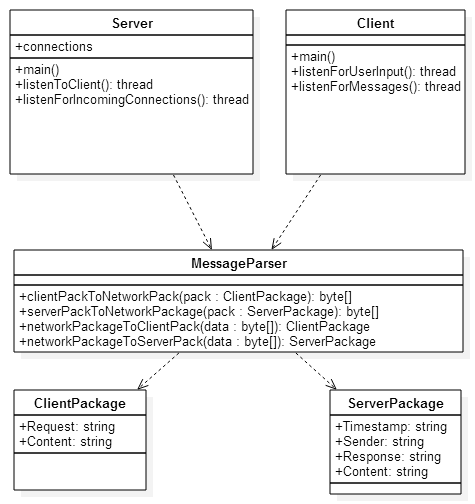
\includegraphics[width=\textwidth]{class_diagram.png}
    \caption{Hovedoppdeling av prosjekt}
    \label{class}
\end{figure}
\section{Sekvensdiagram}
\begin{figure}[H]
    \centering
    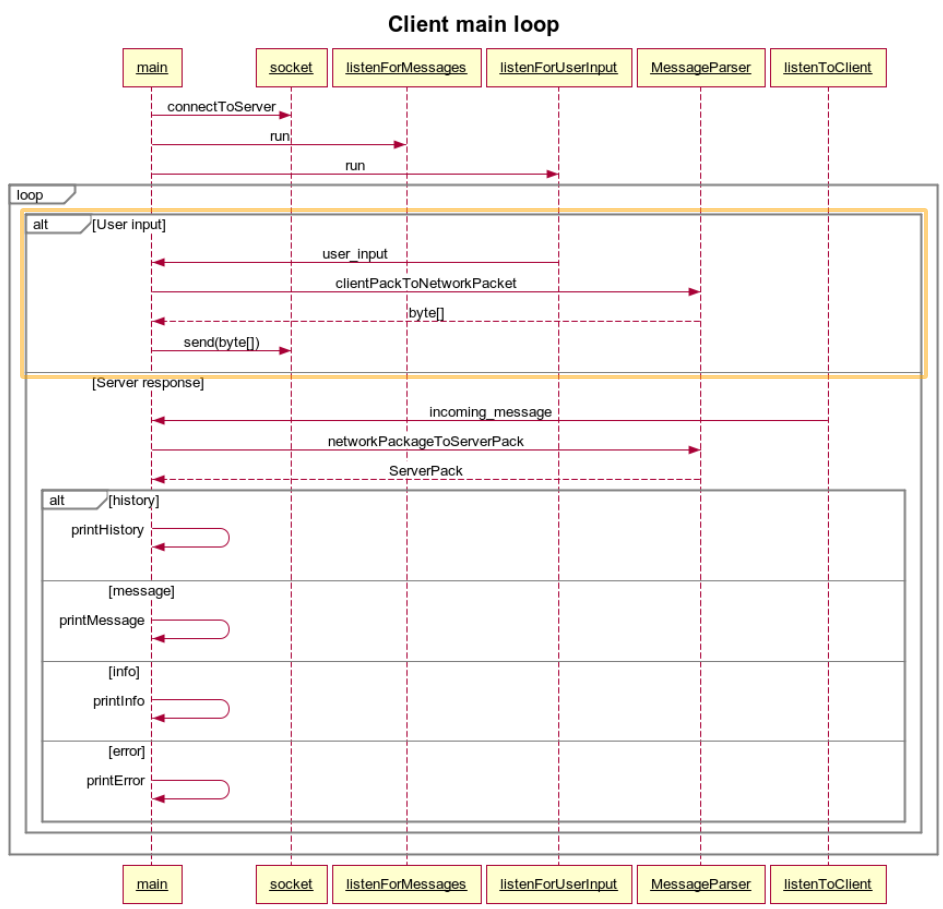
\includegraphics[width=\textwidth]{sequence_client_main.png}
    \caption{Sekvensdiagram for klient}
    \label{seq_client}
\end{figure}

\begin{figure}[H]
    \centering
    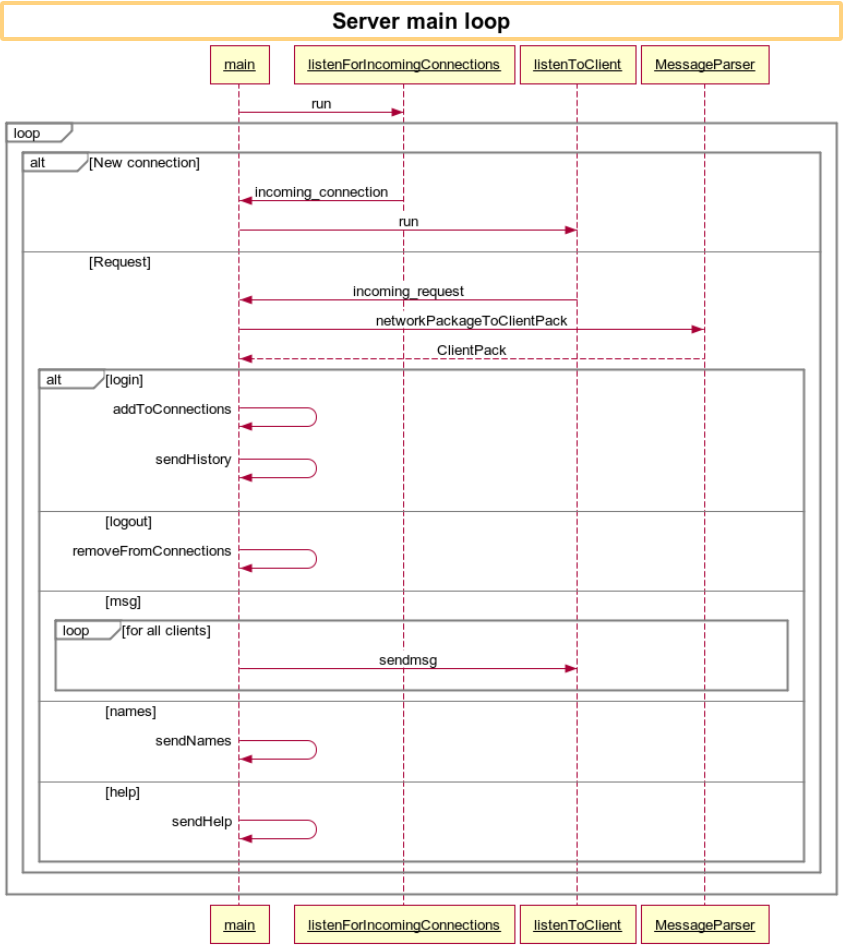
\includegraphics[width=\textwidth]{sequence_server_main.png}
    \caption{Sekvensdiagram for server}
    \label{seq_server}
\end{figure}

\end{document}
